%%%%%%%%%%%%%%%%%%%%%%%%%%%%%%%%%%%%%%%%%
% Beamer Presentation
% LaTeX Template
% Version 1.0 (10/11/12)
%
% This template has been downloaded from:
% http://www.LaTeXTemplates.com
%
% License:
% CC BY-NC-SA 3.0 (http://creativecommons.org/licenses/by-nc-sa/3.0/)
%
%%%%%%%%%%%%%%%%%%%%%%%%%%%%%%%%%%%%%%%%%

%----------------------------------------------------------------------------------------
%	PACKAGES AND THEMES
%----------------------------------------------------------------------------------------

\documentclass{beamer}
\usepackage{hyperref}
\usepackage{listings}

\lstdefinestyle{customc}{
	breaklines=true,
	frame=lines,
	xleftmargin=\parindent,
	basicstyle=\footnotesize\ttfamily,
	keywordstyle=\bfseries\color{blue},
	commentstyle=\itshape\color{orange},
%	numbers=left,
	numberstyle=\tiny,
	identifierstyle=\color{black},
	stringstyle=\color{orange},
}
\lstset{
    %backgroundcolor=\color{white},
    basicstyle=\footnotesize,
    breaklines=true,
    captionpos=b,
    commentstyle=\color{orange},
    extendedchars=true,
    frame=lines,
    keepspaces=true,
    keywordstyle=\color{blue},
    language=c++,
    numbersep=5pt,
    showstringspaces=false,
    style=customc
}
\mode<presentation> {

% The Beamer class comes with a number of default slide themes
% which change the colors and layouts of slides. Below this is a list
% of all the themes, uncomment each in turn to see what they look like.

%\usetheme{default}
%\usetheme{AnnArbor}
%\usetheme{Antibes}
%\usetheme{Bergen}
%\usetheme{Berkeley}
%\usetheme{Berlin}
%\usetheme{Boadilla}
%\usetheme{CambridgeUS}
%\usetheme{Copenhagen}
%\usetheme{Darmstadt}
%\usetheme{Dresden}
%\usetheme{Frankfurt}
%\usetheme{Goettingen}
%\usetheme{Hannover}
%\usetheme{Ilmenau}
%\usetheme{JuanLesPins}
%\usetheme{Luebeck}
\usetheme{Madrid}
%\usetheme{Malmoe}
%\usetheme{Marburg}
%\usetheme{Montpellier}
%\usetheme{PaloAlto}
%\usetheme{Pittsburgh}
%\usetheme{Rochester}
%\usetheme{Singapore}
%\usetheme{Szeged}
%\usetheme{Warsaw}

% As well as themes, the Beamer class has a number of color themes
% for any slide theme. Uncomment each of these in turn to see how it
% changes the colors of your current slide theme.

%\usecolortheme{albatross}
%\usecolortheme{beaver}
%\usecolortheme{beetle}
%\usecolortheme{crane}
%\usecolortheme{dolphin}
%\usecolortheme{dove}
%\usecolortheme{fly}
%\usecolortheme{lily}
%\usecolortheme{orchid}
%\usecolortheme{rose}
%\usecolortheme{seagull}
%\usecolortheme{seahorse}
%\usecolortheme{whale}
%\usecolortheme{wolverine}

%\setbeamertemplate{footline} % To remove the footer line in all slides uncomment this line
%\setbeamertemplate{footline}[page number] % To replace the footer line in all slides with a simple slide count uncomment this line

%\setbeamertemplate{navigation symbols}{} % To remove the navigation symbols from the bottom of all slides uncomment this line
}


\usepackage{graphicx} % Allows including images
\usepackage{booktabs} % Allows the use of \toprule, \midrule and \bottomrule in tables



%----------------------------------------------------------------------------------------
%	TITLE PAGE
%----------------------------------------------------------------------------------------

\title[Group Meeting Talk]{GEM5 Simulator in Full System Mode(3)} % The short title appears at the bottom of every slide, the full title is only on the title page

\author{Yizi Gu} % Your name
\institute[Department of EE,THU] % Your institution as it will appear on the bottom of every slide, may be shorthand to save space
{
Tsinghua University\\ % Your institution for the title page
\medskip
\textit{yizigu@gmail.com} % Your email address
}
\date{\today} % Date, can be changed to a custom date

\begin{document}

\begin{frame}
\titlepage % Print the title page as the first slide
\end{frame}

\begin{frame}
\frametitle{Overview} % Table of contents slide, comment this block out to remove it
\tableofcontents % Throughout your presentation, if you choose to use \section{} and \subsection{} commands, these will automatically be printed on this slide as an overview of your presentation
\end{frame}

%----------------------------------------------------------------------------------------
%	PRESENTATION SLIDES
%----------------------------------------------------------------------------------------

%------------------------------------------------
\section{The Python scripts in GEM5} % Sections can be created in order to organize your presentation into discrete blocks, all sections and subsections are automatically printed in the table of contents as an overview of the talk
\subsection{Python scripts in GEM5}
\begin{frame}
\frametitle{Python scripts in GEM5}
We have known already that Python scripts are involved in GEM5. 

\begin{example}
    \begin{itemize}
	\item For running simulation: fs.py, se.py ,etc.
	\item For configuration: O3\_ARM\_v7a.py, FSConfig.py, etc.
	\item For building simulation objects: Bus.py, Terminal.py,etc.
    \end{itemize}
\end{example}
It is obvious that a Python interpreter has to be called so as to run these scripts. But how is the interpreter called?
\end{frame}

\subsection{How to run Python script in GEM5}
\begin{frame}
\frametitle{Embedding Python in the application}
\begin{block}{src/main.cc}
    \lstinputlisting[language=c++]{main.cc}
\end{block}
\end{frame}
\section{How to add a device}
\subsection{I/O device base classes}
\begin{frame}
\frametitle{Deriving the class from I/O device base classes}
\begin{block}{I/O device base classes}
    \begin{equation*}
	\left.
	\begin{aligned}
	    PIO &: BasicPioDevice\\ 
	    DMA &: DmaDevice 
	\end{aligned}
	\right\}
	\leftarrow PioDevice  \leftarrow MemObject  \leftarrow SimObject
    \end{equation*}
\end{block}
\begin{block}{Create\cite{asplos}}
    \begin{itemize} 
	\item Object header file: src/dev/hellodevice.hh
	\item Object C++ file: src/dev/hellodevice.cc
	\item Parameters file: src/dev/HelloDevice.py
    \end{itemize}
\end{block}
\begin{block}{Modify\cite{asplos}}
    \begin{itemize} 
	\item SConscript: src/dev/SConscript 
	\item Configuration: configs/common/FSConfig.py
    \end{itemize}
\end{block}
\end{frame}
\subsection{Add a I/O device}
\begin{frame}
    \frametitle{Cont'd}
    \begin{block}{src/dev/hellodevice.hh}
	\lstinputlisting[language=c++]{baddev.hh}
    \end{block}
\end{frame}

\begin{frame}
    \frametitle{Cont'd}
    \begin{block}{src/dev/HelloDevice.py}
	\lstinputlisting[language=python]{BadDevice.py}
    \end{block}
\end{frame}

\begin{frame}
    \frametitle{Cont'd}
    \begin{block}{Change in FSConfig.py}
	\lstinputlisting[linerange=272-278]{/home/gyz/code/architecture/fullsys/gem5-stable-fs/configs/common/FSConfig.py}
    \end{block}
\end{frame}

\begin{frame}
    \frametitle{Writing relevant driver}
    Requesting hte I/O port using {\it request\_region} function
    \begin{block}{}
	\lstinputlisting[language=c++]{/home/gyz/code/os/driver/test/baddev/dev.c}
    \end{block}
\end{frame}

\begin{frame}
    \frametitle{Problem encountered}
    After insmod, the system complains that the device is not found:
    \begin{figure}[H]
	\begin{center}
	    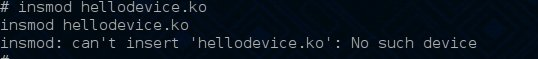
\includegraphics[width=.8\textwidth]{m10.jpg}
	\end{center}
    \end{figure}
\end{frame}

\begin{frame}
    \frametitle{Reference}
    \begin{thebibliography}{99}
	    \bibitem{asplos}
	    Ali Saidi,et al,
	    \emph{Using the M5 Simulator ASPLOS XIII}.
    \end{thebibliography}
\end{frame}
\begin{frame}
\Huge{\centerline{Thank you}}
\end{frame}


\end{document} 
\end{document}
